\documentclass[10pt]{llncs}

\usepackage[T1]{fontenc}
\usepackage[utf8]{inputenc}
\usepackage[a4paper,margin=2cm,top=1.5cm,bottom=1.5cm]{geometry}
\usepackage{graphicx}
\usepackage{hyperref}
\usepackage{url}
\usepackage{amsmath}
\usepackage{booktabs}
\usepackage{multirow}
\usepackage{xcolor}
\usepackage{setspace}
\usepackage{times}
\usepackage{microtype}
\singlespacing
\setlength{\columnsep}{0.25in}
\setlength{\emergencystretch}{1em}

\begin{document}

\title{AI-Powered Movie Recommendation Platform with Cloud-Native Microservices}

\subtitle{Group 03 - Platforms for AI Systems}

\author{
    \parbox{\textwidth}{
        \centering
        Martim Aires de Sousa (ist1106468)\inst{1}\\
        {\small \texttt{martim.aires.de.sousa@tecnico.ulisboa.pt}}\\[0.8em]
        Cristiano Pantea (ist1XXXXXX)\inst{1}\\
        {\small \texttt{[email]}}\\[0.8em]
        João Pinheiro (ist1XXXXXX)\inst{1}\\
        {\small \texttt{[email]}}
    }
}

\institute{Departamento de Engenharia Informática, Instituto Superior Técnico}

\twocolumn[\maketitle\vspace{5em}]

\section*{Abstract}
This project presents the design and deployment of an AI-powered movie recommendation platform built as a microservice-based system. The application enables user authentication, profile management, personalized recommendation generation, and cached recommendation delivery in a cloud-native environment. The system integrates Keycloak for identity management, Flask services for business logic, PostgreSQL for persistent storage, Redis for caching, and Ollama for local model inference. The platform is deployed both locally with Docker Compose and in a Kubernetes environment using Helm charts, custom manifests, Terraform, and Ansible automation.

The project addresses the requirements of a realistic distributed application in which multiple services cooperate to provide a functional user experience while ensuring observability and operational traceability. In addition, the solution includes persistent storage for selected services, an advanced deployment feature described in the project requirements. The result is a reproducible environment for experimentation, benchmarking, and demonstration of an AI-enabled recommendation service in a microservice architecture.

\section{Introduction}

Modern recommendation systems increasingly rely on distributed architectures to separate user interfaces, data management, model inference, and monitoring concerns. In this context, microservices provide modularity and independent deployment. This project follows that paradigm by implementing a movie recommendation platform that combines authentication, profile management, AI-based suggestion generation, and persistent data storage in a complete system.

The goal is to provide a simple but functional application that allows users to register, log in, define their preferences, and receive personalized recommendations aligned with both their interests and the movie catalog. In addition, the system includes a proactive cache component that generates recommendations in advance so that users see relevant results quickly after login.

The project is implemented as a realistic cloud-native application and is organized according to the specification defined for this project. It emphasizes reproducibility and deployability, while also supporting a monitoring and observability layer suitable for evaluating service health and request latency.

\section{System Design and Architecture}

The application is structured as several independent services connected through HTTP interfaces and environment-based configuration. The main components are:

\begin{figure*}[t]
    \centering
    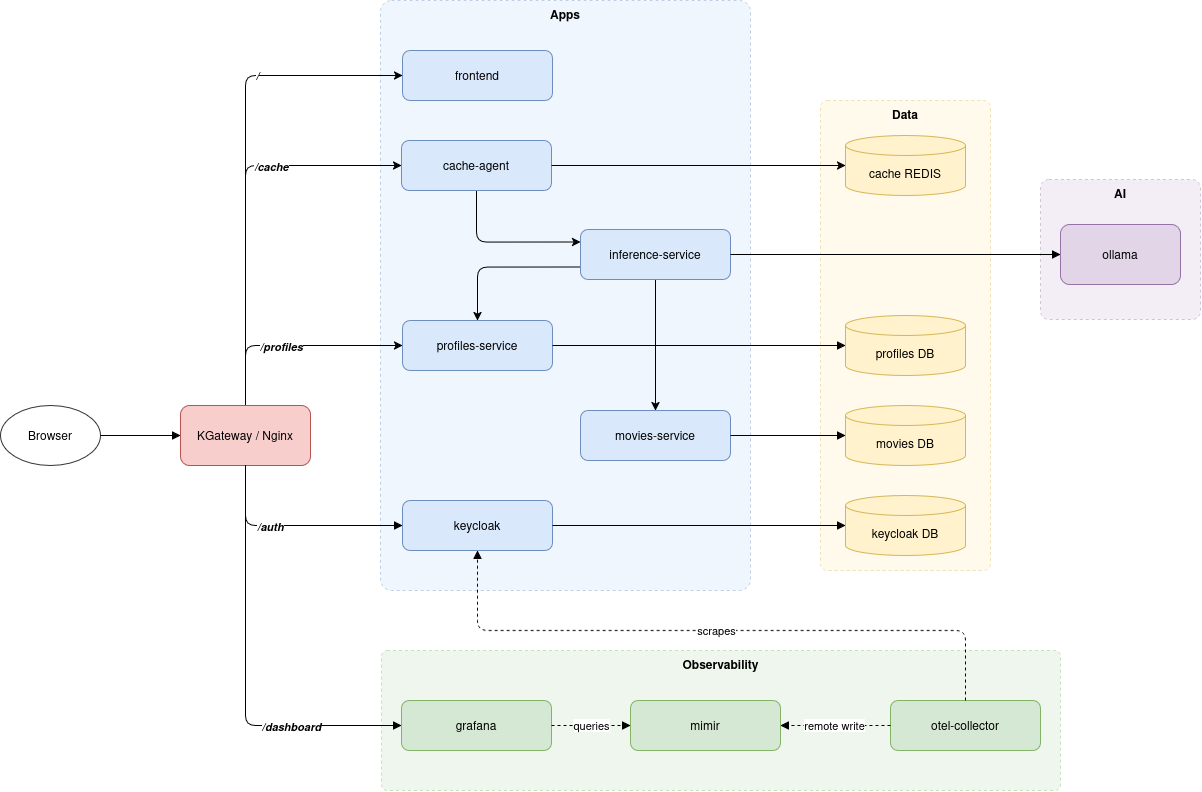
\includegraphics[width=\linewidth]{static/architecture.drawio.png}
    \caption{Overview of the microservice architecture for the movie recommendation platform.}
\end{figure*}

\begin{itemize}
    \item \textbf{Frontend:} a web interface developed with React and Vite, used for authentication and interaction with the recommendation system.
    \item \textbf{Authentication:} Keycloak provides identity management and token validation for secure access across microservices.
    \item \textbf{Profiles service:} stores user profiles, favorite genres, watch history, and mood information in a PostgreSQL database.
    \item \textbf{Movies service:} provides the movie catalog and metadata used to improve the recommendations' quality. The goal is for the inference service to rank cataloged movies.
    \item \textbf{Inference service:} invokes a local language model through Ollama to generate recommendation results based on user preferences.
    \item \textbf{Cache agent:} stores up-to-date recommendations for each user (in Redis) for fast retrieval and warm-start experience.
    \item \textbf{Monitoring stack:} Grafana, Mimir, and OpenTelemetry provide metrics and dashboards for observability.
\end{itemize}

The \textbf{frontend} communicates with backend microservices through authenticated (\textbf{Keycloak} produces and verifies tokens for users' requests) REST endpoints rather than relying on a monolithic backend. Each service has a clearly defined responsibility, with service-to-service communication handled through authenticated HTTP requests and environment-based routing.

The \textbf{Profiles Service} handles profile-related operations, allowing users to view and update their profiles and explore those of other users. The \textbf{Inference Service} generates recommendations on demand by retrieving the user's profile and matching movies from the \textbf{Movies Catalog Service}. It then combines this information into a structured prompt and sends it to the LLM to generate personalized recommendations.

The \textbf{Cache Service} provides cached recommendations for faster responses. A background agent asynchronously refreshes recommendations and stores them in Redis, reducing latency and avoiding unnecessary inference requests.

For observability, Keycloak exposes metrics collected by \textbf{OpenTelemetry}, while the Inference Service pushes telemetry data to the observability stack. \textbf{Mimir} stores the collected metrics, and \textbf{Grafana} queries Mimir to visualize them through dashboards, enabling centralized monitoring of authentication and recommendation workloads.

This architecture promotes loose coupling, independent deployment and scaling, improved performance, and fault isolation across the recommendation workflow. In practice, the platform relies on Keycloak for user authentication and identity federation. The frontend authenticates through the Keycloak JavaScript client, while the backend services validate JSON Web Tokens using the Keycloak JWKS endpoint. This ensures that access to user-specific profile information and recommendation endpoints remains protected.

The profiles service stores the user state in PostgreSQL and exposes endpoints to retrieve and update the active profile. User data includes favorite genres, disliked genres, actors, mood, watch history, and profile visibility. Input validation is performed to maintain consistency and avoid malformed data. The inference service acts as the orchestration layer between the profiles service, movie catalog, and LLM. It retrieves candidate movies, filters out previously watched titles and undesired genres, and constructs a recommendation request based on the profile. The local model then ranks the candidate list and returns a structured set of movie suggestions.

The cache agent is responsible for storing and refreshing recommendation data. When a profile is updated, the service triggers a re-evaluation of recommendations and stores the result in Redis. This allows the application to provide immediate personalized recommendations when users log in, reducing the delay associated with generating recommendations from scratch. This mechanism significantly improves responsiveness and is especially useful in a recommendation system where users expect quick results after authentication.

The system integrates telemetry collection and dashboards to support operational visibility. Metrics from service execution and infrastructure health are exported through OpenTelemetry and centralized in Grafana and Mimir. This enables tracing of user requests, evaluation of service health, and identification of bottlenecks in the architecture.

\section{Advanced Components and Deployment Methods}

One of the advanced deployment options described in the project specification is the use of persistent storage. The implemented solution includes persistent volumes for the main stateful services, namely Keycloak PostgreSQL, the profiles service database, and the Redis cache database. This ensures that data remains available across restarts and is not lost after a temporary infrastructure interruption.

This feature is particularly relevant in a cloud-native application because it provides a more robust operational baseline and aligns with deployment practices expected in a realistic production environment. It also directly addresses the requirement that the system remain functional even after infrastructure restart events.

In addition to persistence, the project relies on Kubernetes and Helm-based deployment automation, Docker Compose for local experimentation, and observability tooling for operational monitoring. This composition of advanced deployment methods demonstrates a realistic, reproducible environment for microservice orchestration and validation. The project supports both local and Kubernetes-based deployment: Docker Compose is used for rapid local experimentation, while Helm charts and custom manifests orchestrate the cluster deployment. This multi-environment strategy addresses a key project requirement by ensuring that the solution remains reproducible and realistic while enabling validation under different infrastructure conditions.

\section{Evaluation and Performance Study}

The project statement requires a system evaluation including throughput and latency as the number of concurrent clients grows. This evaluation is essential to understand how the application behaves under load and which components become performance bottlenecks.

The proposed evaluation methodology is as follows:

\begin{enumerate}
    \item Define a workload representative of the recommendation workflow, including login, profile retrieval, and recommendation request generation.
    \item Increase the number of concurrent clients gradually from 1 to 50 or higher.
    \item Measure average response time, p95 latency, and throughput in requests per second.
    \item Record the behavior of the authentication, profiles, inference, and cache layers under increasing load.
\end{enumerate}

\begin{table*}[t]
\centering
\begin{tabular}{p{2.6cm}p{2.2cm}p{2.2cm}p{2.5cm}p{3.4cm}}
\toprule
Concurrent clients & Avg. latency (ms) & p95 latency (ms) & Throughput (req/s) & Observation \\
\midrule
1 & [value] & [value] & [value] & Baseline \\
10 & [value] & [value] & [value] & Stable \\
25 & [value] & [value] & [value] & Minor degradation \\
50 & [value] & [value] & [value] & Increased latency \\
100 & [value] & [value] & [value] & Saturation region \\
\bottomrule
\end{tabular}
\caption{Representative load-test measurements.}
\end{table*}

The expected bottleneck is the AI inference layer because recommendation generation requires model execution and may be slower than the profile and cache operations. Nevertheless, cache hits and filtered candidate selection can reduce latency in repeated requests. This evaluation helps quantify the trade-off between recommendation quality and system responsiveness. Overall, the project demonstrates a realistic AI-powered recommendation platform that satisfies the base microservice requirements while incorporating advanced persistence and deployment features in a reproducible cloud-native environment.

\end{document}


% TODO:
% - Cloud init (storage class; CSI drivers; updated k8s version to use helm charts to the latest version of the charts)
% - All different environments
% - Explain better each service (helm charts, etc...)
% - Terraform and Ansible usage
